\chapter{Messungen und Experimente}
\label{cha:experiments}
Im Verlauf der Entwicklung des XenoFlow Lastverteilers sind immer wieder Behauptungen seitens NVidia aufgetaucht, die sehr vielversprechend klangen. Um die Leistung der BlueField-3 jedoch genauer beschreiben zu können und zu überprüfen, ob die Behauptungen so auch reproduzierbar sind, wurden mehrere Experimente auf der Karte durchgeführt und diverse Messungen gemacht. Im folgenden Abschnitt werden die Ergebnisse und Messaufbauten vorgestellt.
\section{Forschungsfragen}
In Zusammenarbeit mit der Arbeitsgruppe wurden 3 Fragen in den Vordergrund gestellt. Alle diese 3 sind direkt dem Marketingmaterial von NVidia entnommen und sollen sicherstellen, dass die Karte in möglichst vielen Situationen die gewünschte und proklamierte Leistung erreicht.
\begin{itemize}
    \item Ist das Versprechen von Zero-Overhead-Verarbeitung ohne Paketverlust aus der NVidia Dokumentation so wahrheitsgetreu?
    \item Ist es tatsächlich möglich, auch unabhängig von der Paketgröße, immer die angegebenen 400 Gbit/s zu verarbeiten?
    \item Inwiefern beeinflusst die Last des Load-Balancers die Round-Trip-Time, also somit die Latenz?
\end{itemize}
\section{Messaufbau}
Um die Leistung eines Lastverteilers zu quantifizieren, sollte ein möglichst realistisches Szenario für Messungen verwendet werden. Ein denkbares und für diese Arbeit verwendetes Szenario wäre ein Lastverteiler für eingehende UDP-DNS-Requests. Ein DNS-Server stellt normalerweise IP-Adressen bereit, die auf einen entsprechenden Server zeigen. Diese IP-Adresse ist mit einer entsprechenden Domain verbunden. Möchte nun also ein Client auf einen bestimmten Server unter einer Domain zugreifen, so stellt er einen DNS-Request an einen DNS-Server. Da auf diesen Server nun für jede Domain, die aufgelöst werden soll, ein Request eintrifft, ist mit einer Menge von Clients schnell die entsprechende maximale Leistungsfähigkeit des DNS-Servers erreicht. Hier setzen wir nun einen Lastverteiler ein, damit die entsprechenden Requests nicht von einem einzelnen Server beantwortet werden, sondern von einer Reihe von Servern, die jeweils die gleichen Daten an Domain-IP-Adressen-Kombinationen hinterlegt haben. Dieser Lastverteiler ist in unserem Fall der XenoFlow. Dazu sind in einem eigens dafür abgestellten Testnetzwerk fünf Knoten verbunden. Vier dieser Knoten besitzen eine entsprechende Infiniband-Netzwerkkarte, die es ihnen erlaubt, mit 100 Gbit/s Netzwerkverkehr zu verarbeiten. In dem fünften Knoten \textbf{fips-5} ist die BlueField-3 verbaut. Damit die entsprechenden richtigen Backends angesprochen werden können, wurden auf dem Switch, der die Server miteinander verbindet, die entsprechenden MAC-Adressen an die Hardwareports per Konfiguration gebunden.
\subsection{Knoten}
Folgende Knoten mit ihrer entsprechenden Funktion kamen zum Einsatz:
\begin{itemize}
    \item \textbf{fips1} - Stellt den Testclient dar, der im folgenden UDP-DNS-Requests an den Server sendet.
    \item \textbf{fips2} - Backend Server, auf dem sowohl Grundlast ankommt als auch der DNS-Server läuft.
    \item \textbf{fips3} - Backend Server, auf dem nur Grundlast ankommt.
    \item \textbf{fips4} - Lasterzeugender Server
    \item \textbf{fips5} - XenoFlow Knoten, in dem die BlueField-3 verbaut ist.
\end{itemize}
Die fips* Knoten sind mit jeweils zwei Intel Xeon Silver 4514Y Prozessoren ausgestattet. Diese besitzen jeweils 16 Kerne, womit ein Knoten auf 32 Kerne mit 64 Threads kommt. Die Prozessoren des Hosts besitzen einen Basistakt von 2 GHz und Turbotakt von 3.4 GHz. Außerdem besitzen die Knoten 128 GB DDR4 Arbeitsspeicher. Sie sind mittels Mellanox ConnectX Kabeln verbunden. Die BlueField-3 hat einen ARM-Cortex-A78AE mit 16 Kernen verbaut. Dieser hat einen Takt von 2.4 GHz. Die BlueField-3 hat außerdem 32 GB DDR4 Arbeitsspeicher verbaut. Zusätzlich besitzt die Karte einen Co-Prozessor (Data Path Accelerator) der RISC-V Architektur. Genauer kommt dieser auf einen Basistakt von 1.8 GHz. Letzterer ist vor allem für diese Messreihe relevant. 
\subsection{Trafficgenerator}
Um Traffic von einem einzelnen Knoten zu generieren, der möglichst nahe an realistischem Netzwerkverkehr liegt, kam im Zuge dieser Arbeit der T-Rex-Trafficgenerator zum Einsatz. Dieser ist vollständig Open Source. TRex verwendet direkt DPDK, was es ihm ermöglicht, eine sehr große Anzahl von Netzwerkverkehr zu erzeugen, ohne einen großen Overhead auf dem entsprechenden lastgenerierenden System zu erzeugen. Es werden diverse Protokolle unterstützt, wie ARP, IPv6, TCP/UDP und DNS. In den folgenden Versuchsreihen wurde die Grundlast durch ein entsprechendes Pythonskript erzeugt, welches direkt mit der TRex API arbeitet. Das Skript befindet sich ebenfalls im Repository dieser Arbeit.
\subsection{DNS-Server}
Damit Messungen wie die Latenz oder der Paketverlust durchgeführt werden können, bedarf es eines kleinen DNS-Servers, der die Client-Requests beantwortet. Dazu wurde abermals ein kleiner Server in Python implementiert, der auf ein Request für eine Domain-Adresse mit der zugehörigen IP-Adresse antwortet. Auch hierbei ist der entsprechende Serverquellcode im Repository der Arbeit hinterlegt.
\section{Messungen}
Der XenoFlow LoadBalancer ist aktuell in der Lage, UDP-Pakete, die an ihn per MAC-Adresse gerichtet sind, zu einer Reihe von zugeordneten Backends weiterzuleiten. Folgende Metriken sollen dabei gemessen werden: 
\begin{itemize}
    \item Packet Rate (PPS - Packets per Second)
    \item Latenz (RTT - Round Trip Time)
    \item Packet Loss (\%)
\end{itemize}
Zur Messung der Packet Rate und des Packet Losses wird ethtool verwendet, da es so möglich ist, Hardwarestatistiken beziehen zu können, die direkt von der Hardware bereitgestellt werden und somit nicht erst vom Linux-Kernel verarbeitet werden müssen.
\begin{figure}
    \centering
    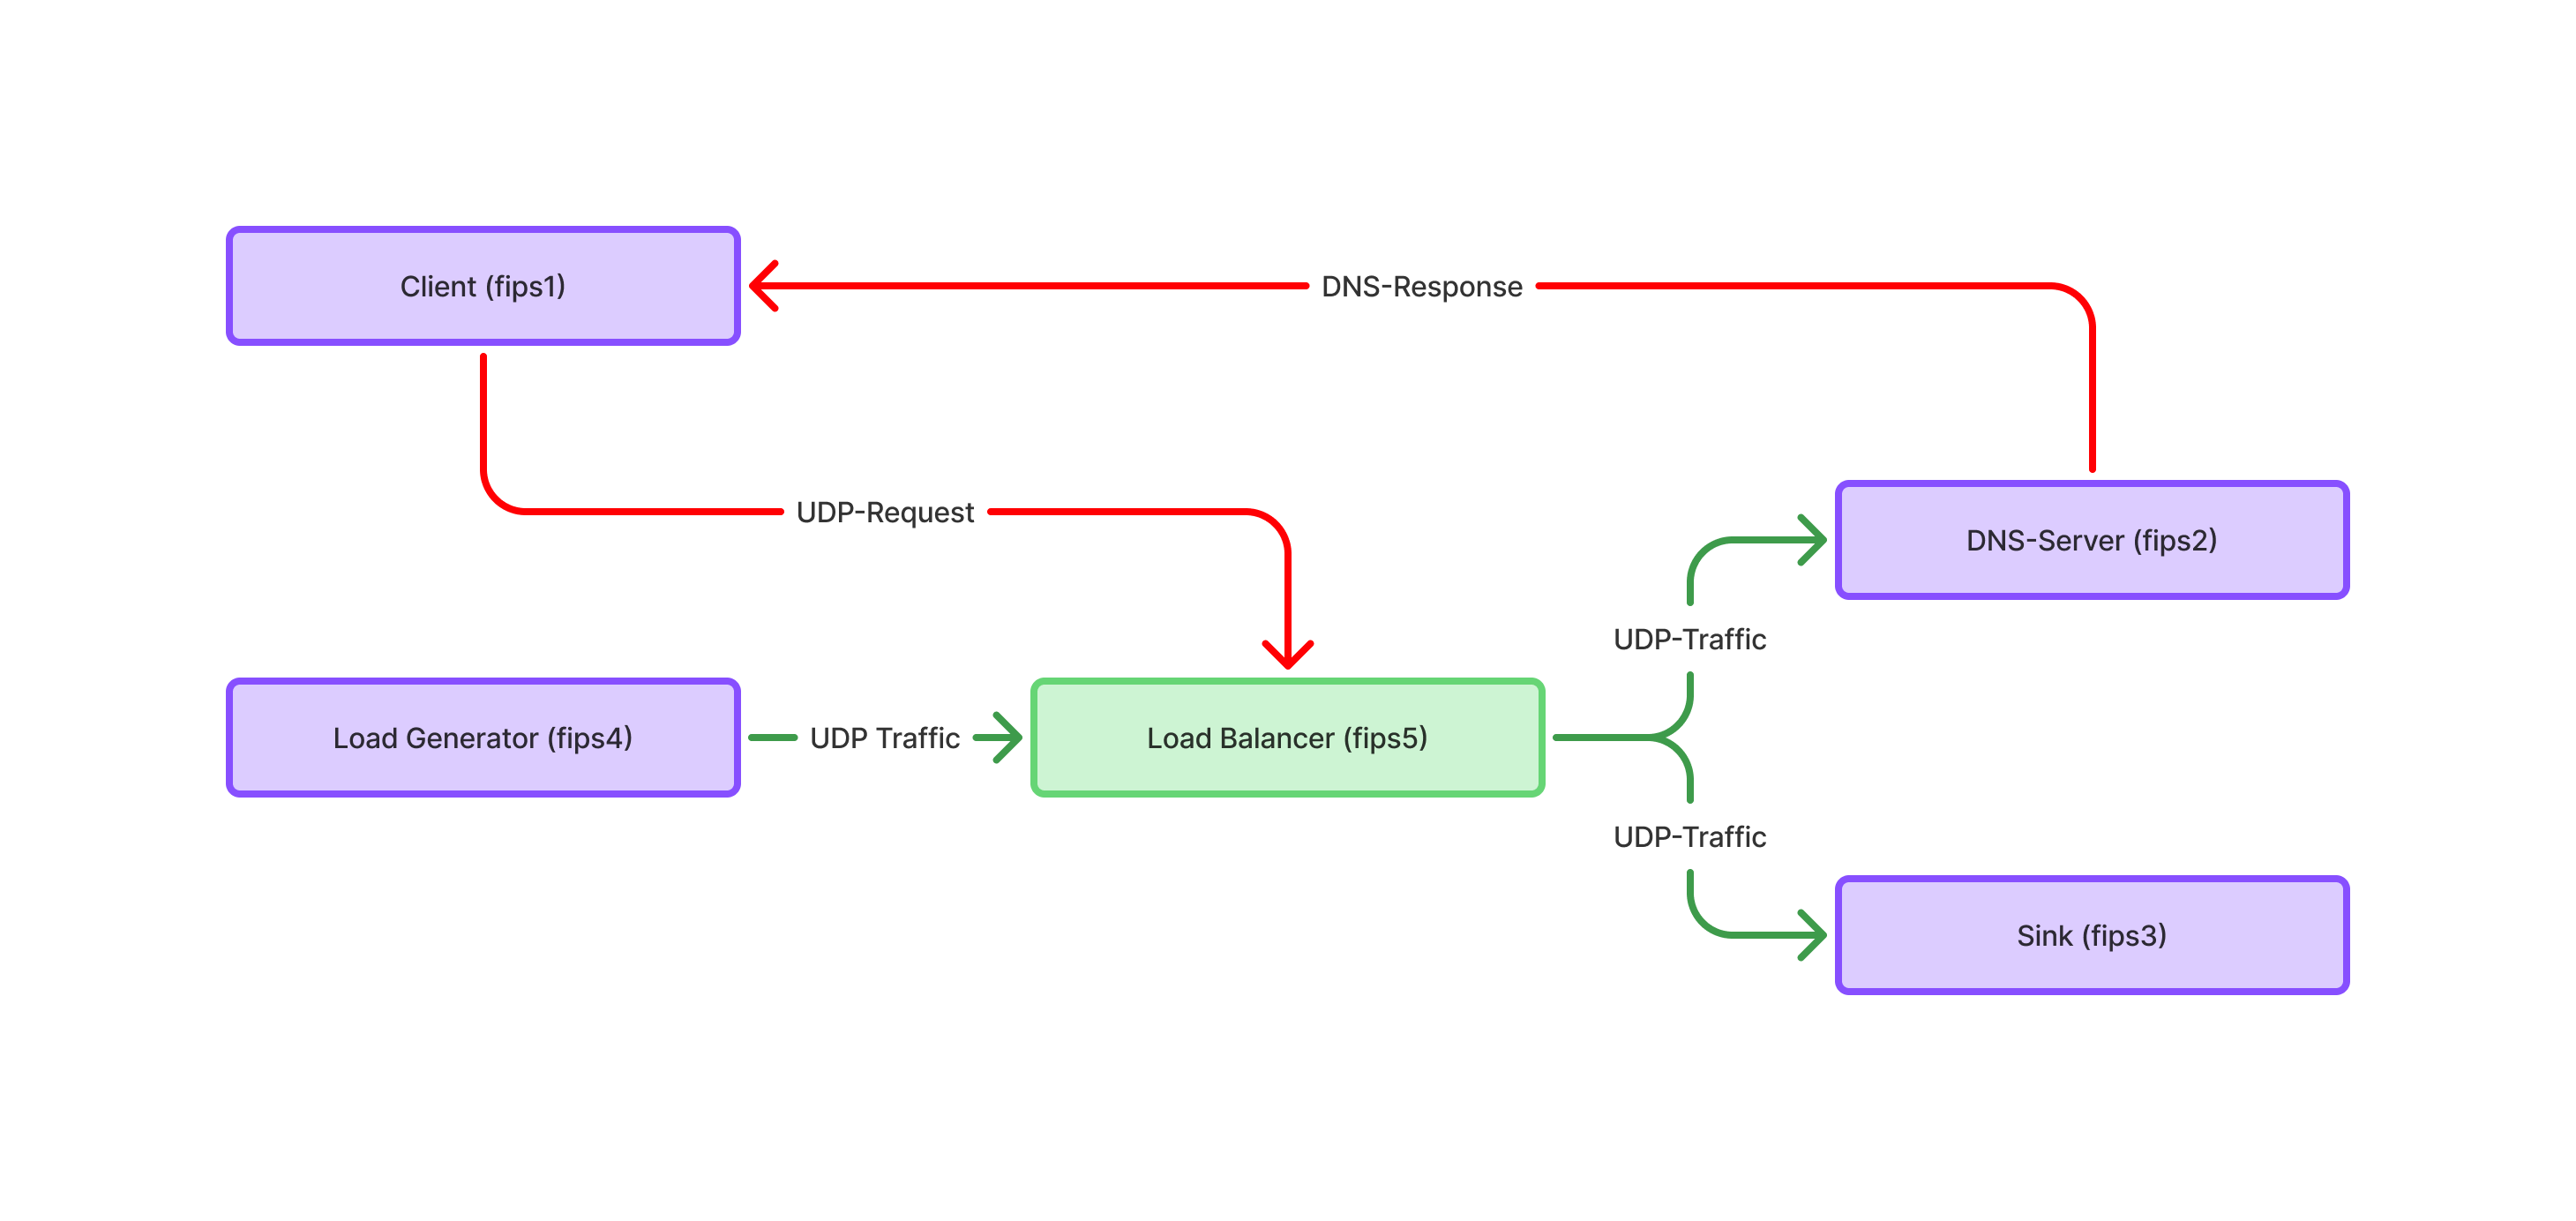
\includegraphics[width=1\linewidth]{images/Messaufbau Latenz.png}
    \caption{Latenz- und Paketloss-Aufbau}
    \label{fig:enter-label}
\end{figure}
\begin{figure}
    \centering
    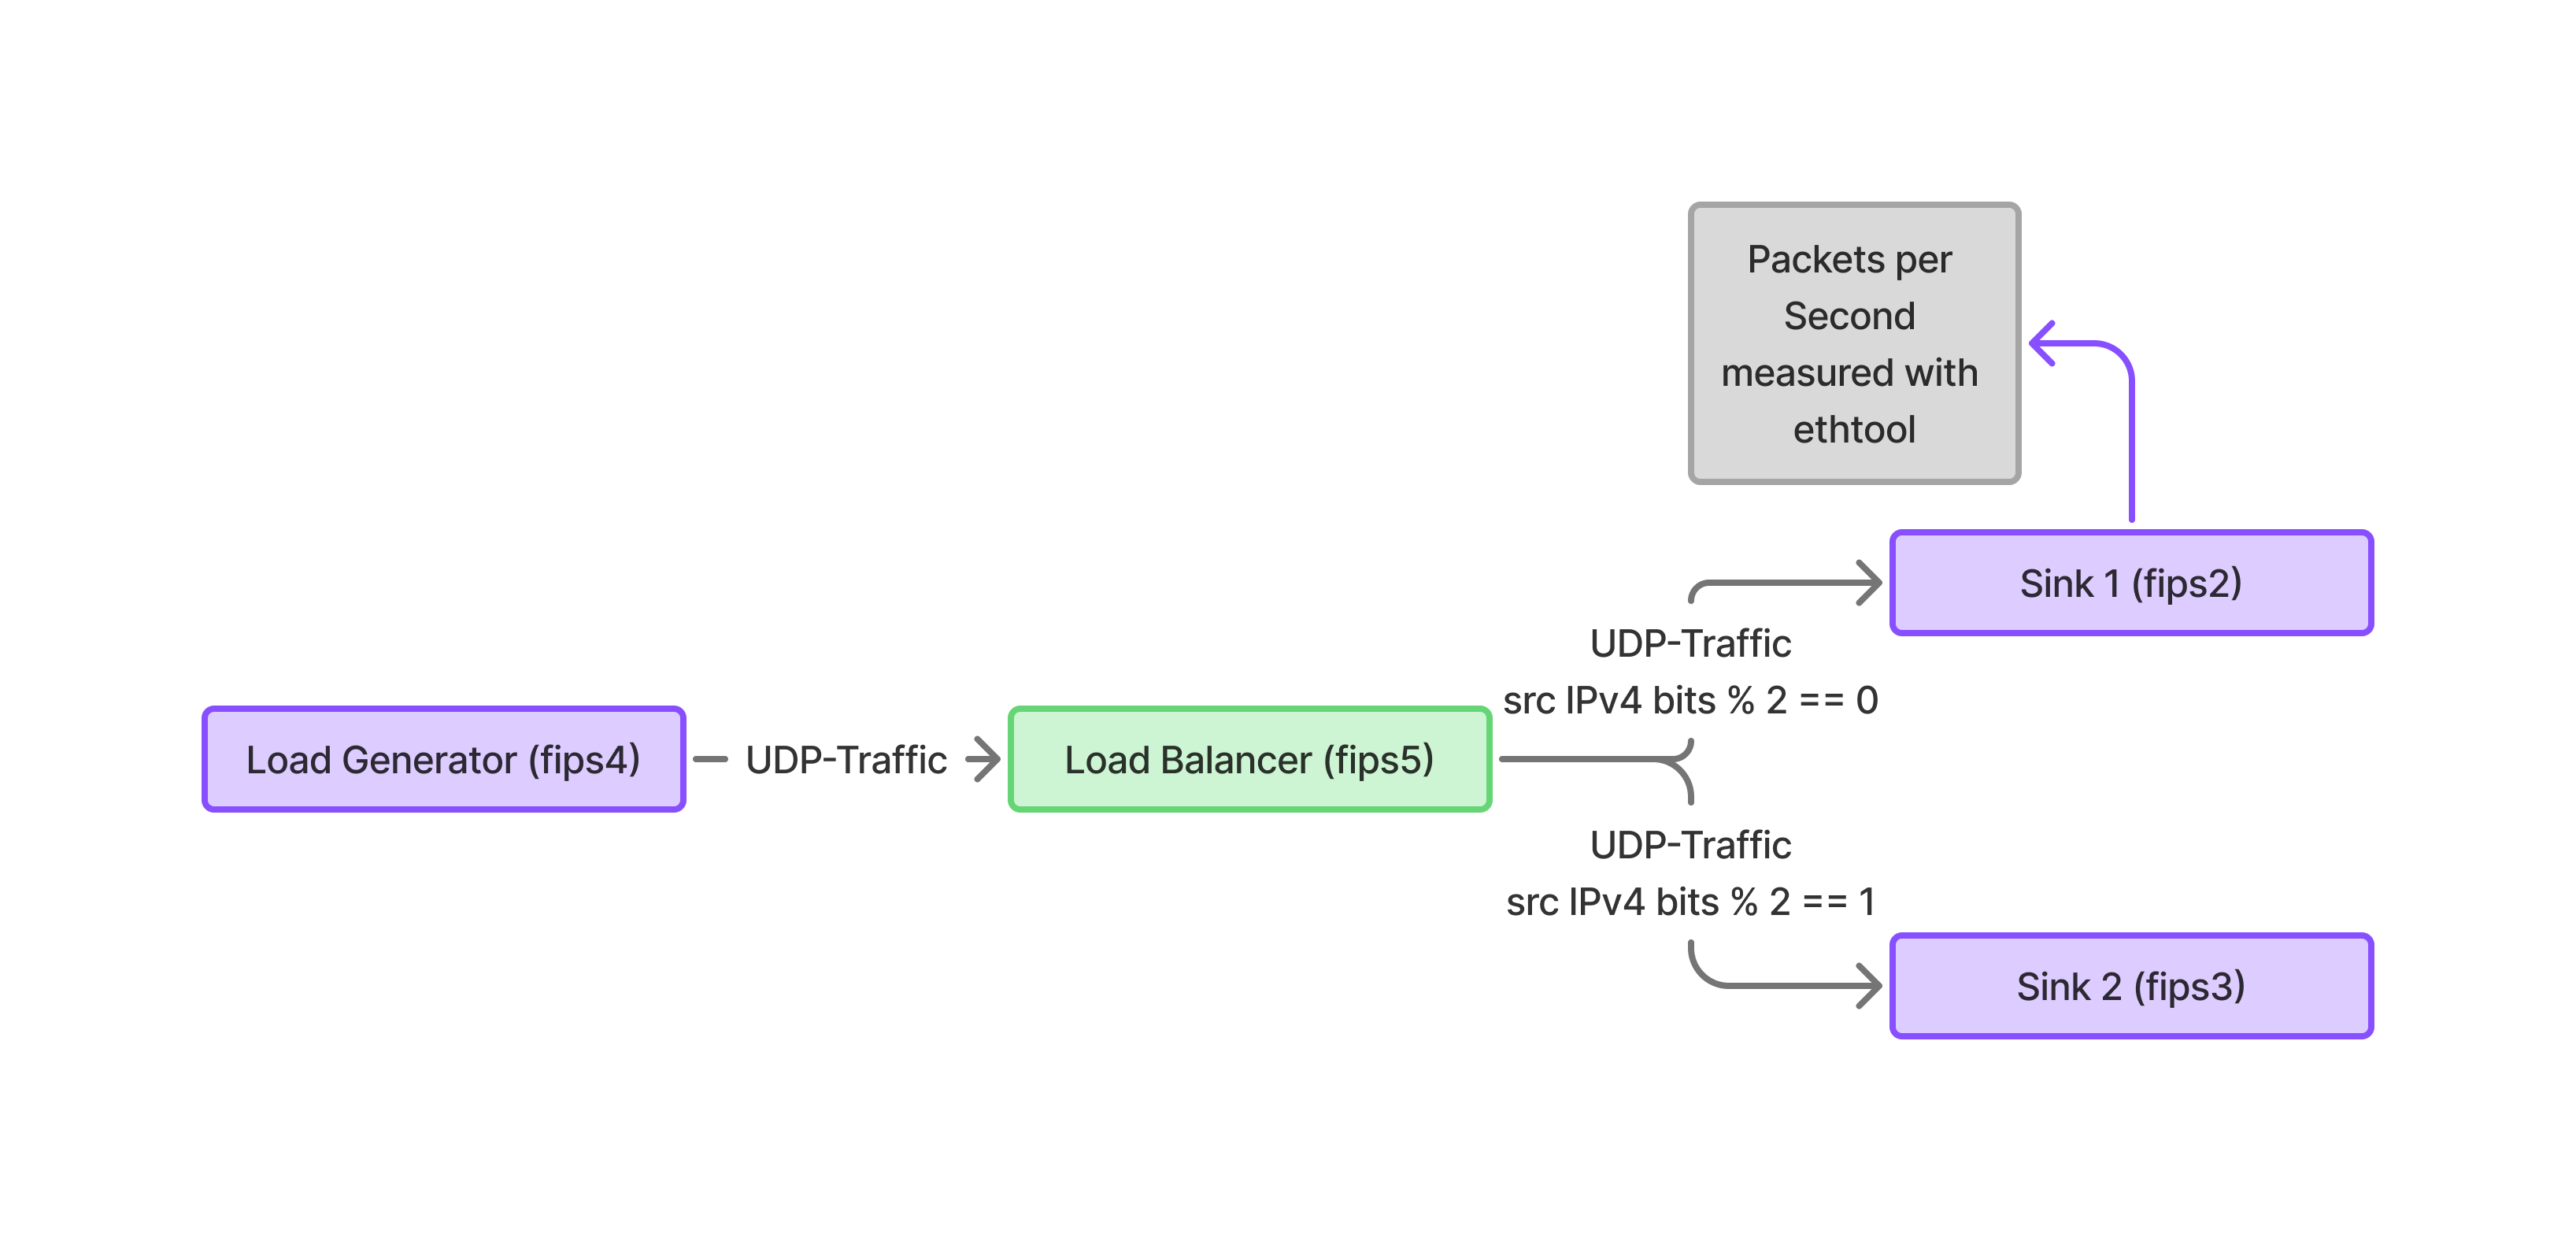
\includegraphics[width=1\linewidth]{images/Messaufbau PPS.png}
    \caption{Paketdurchsatzmessungs-Aufbau}
    \label{fig:enter-label}
\end{figure}
\subsection{Packet Rate}
Bei der Paketrate wird in Abhängigkeit von der Paketgröße gemessen, ob sich der maximale mögliche Paketdurchsatz ändert. Dieser Durchsatz wird hierbei in Paketen pro Sekunde gemessen. Die Variable, die verändert wird, ist hierbei die Paketgröße. Somit erhalten wir daraufhin einen Plot, in dem an der Abszisse die Paketgrößen abgetragen sind und an der Ordinate die Anzahl an maximal möglichen Paketen pro Sekunde. Zusätzlich zu den abgebildeten Paketgrößen wurde eine Basismessung durchgeführt, bei der gar keine Last auf dem Load-Balancer wirkt (siehe Abbildung 7.2).
\subsection{Latenz}
Bei der Latenzmessung wird der Laufzeitzuwachs durch die Verarbeitung des XenoFlow LoadBalancers gemessen. Die Messgröße ist hierbei eine Zeiteinheit in Millisekunden oder Mikrosekunden. Die Variable, die verändert wird, ist abermals die Paketgröße, um sicherzustellen, dass die Hardwarebeschleunigung tatsächlich auf der Ebene des Bitfeldes rechnet. Dazu wird in der Auswertung dann ein Plot erstellt, in dem Paketgröße und Latenzzuwachs aufgetragen sind (siehe Abbildung 7.1).
\subsection{Packet Loss}
Der Packet Loss misst, zu welchem Zeitpunkt und vor allem wie viele Pakete bei einer bestimmten Last auf dem LoadBalancer verloren gehen. Die gemessene Metrik ist hierbei ein Prozentsatz, der angibt, wie viel anteilshaft vom tatsächlichen Traffic auch vom LoadBalancer verarbeitet werden kann. Die Variable, die hierbei variiert wird, ist die Last auf den Load-Balancer. Dabei wird die Anzahl der Pakete pro Sekunde variiert. In der Auswertung wird ähnlich wie bei der Latenz der Grundtraffic dem Packet Loss gegenübergestellt.
\section{Ergebnisse}
Zunächst war das formulierte Ziel, eine vollständige Hardwarebeschleunigung seitens der BlueField-3 verwenden zu können, um den Traffic zu verarbeiten. Dies war leider zunächst so nicht möglich. Die ersten Versuche zeigten durch die sichtbare CPU-Last auf dem BlueField-System deutlich, dass der Netzwerkverkehr nicht vollständig über die Hardwareeinheiten geleitet wurde. Das war doch sehr verwunderlich, da in keinem uns bekannten Abschnitt der Dokumentation von einer speziellen Konfiguration oder Ähnlichem die Rede war, die diese Funktion aktiviert. Nach einer Weile und vielen Versuchen entstand allerdings die Idee, mittels Open vSwitch den Netzwerkverkehr derart umzuleiten, dass alle Pakete, die auf \textbf{Port 0} eintreffen, direkt auf \textbf{Port 1} weitergeleitet werden. Nachdem diese Konfiguration mittels des Open vSwitch CLI-Tools vorgenommen wurde, verschwand die Last auf den ARM-Kernen der BlueField sofort. Wurde nun der Lastverteiler gestartet, so war ebenfalls keine Last mehr auf den Kernen zu beobachten. Somit liegt die Vermutung nahe, dass nun der Netzwerkverkehr auf der ASIC-Hardware verarbeitet wurde. Außerdem werden so Mutmaßungen über die Architektur der BlueField-3 möglich. Es ist sehr wahrscheinlich, dass DOCA-Flow-Applikationen wirklich auf der ASIC-Hardware ausgeführt werden und somit ein Off-Path-Switching umsetzen, da weder auf Port-0 noch Port-1 auf dem Betriebssystem der BlueField-3 Pakete beobachtet werden können. 
\subsection{Packet Rate}
Bei dem Versuch der Packet Rate wurde gemessen, wie viele Pakete pro Sekunde von der BlueField-3 verarbeitet werden können.
\begin{figure}
    \centering
    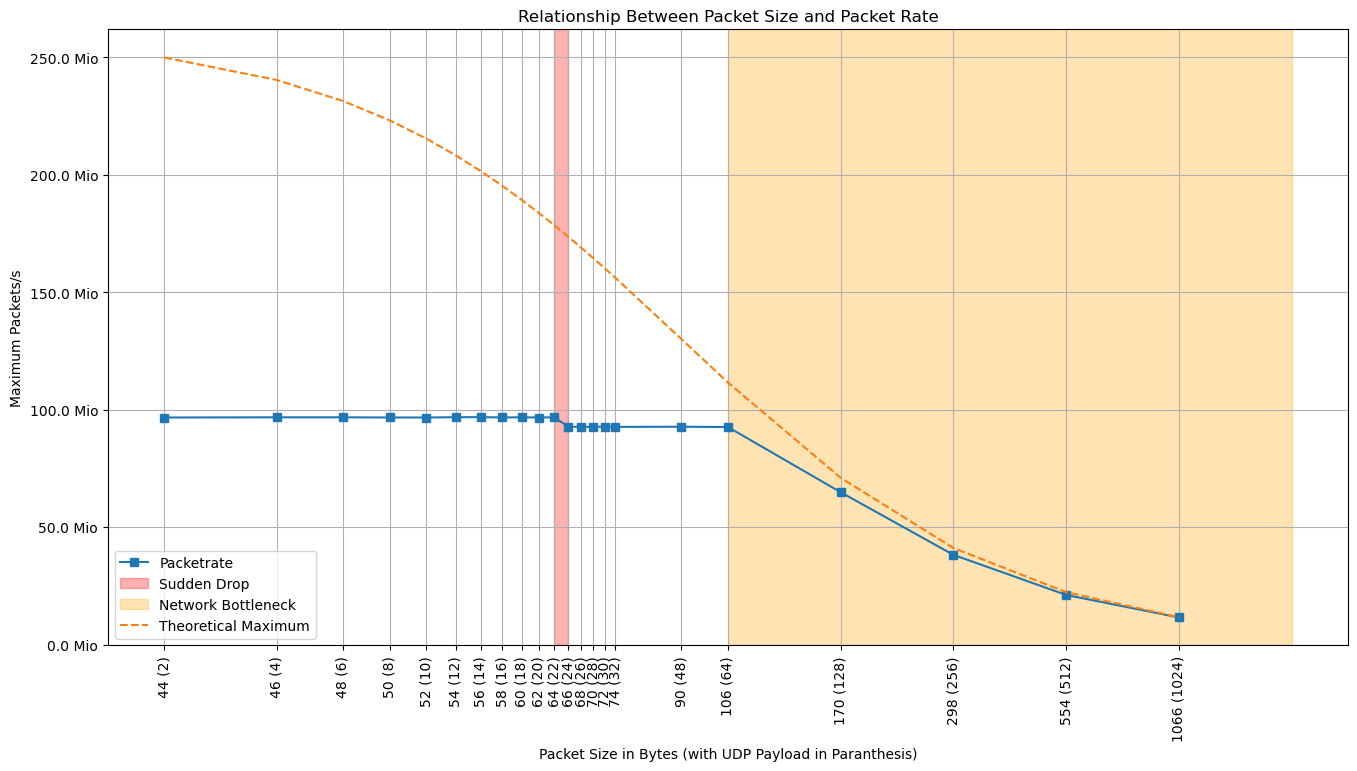
\includegraphics[width=1\linewidth]{images/pps_pps.png}
    \caption{Pakete pro Sekunde - variierende Paketgröße}
    \label{fig:enter-label}
\end{figure}
Dabei wurde die Paketgröße variiert, indem die Größe der UDP-Payload geändert wird. Sollte nun die Größe der Pakete des Netzwerkverkehrs einen Einfluss darauf haben, wie viele Pakete verarbeitet werden können, so würde sich hier eine Kurve entsprechend abzeichnen. Dies ist so nicht der Fall (siehe Abbildung 7.2). Gemessen wurden UDP-Payloadgrößen von 2 bis 1024 Bytes. Zunächst ist zwischen 2 und 22 Bytes keine Veränderung der möglichen Paketrate sichtbar. Es werden konstant ca. 98 Millionen Pakete pro Sekunde vom Loadbalancer verarbeitet und können auf dem entsprechenden Backend beobachtet werden, auf dem die Pakete ankommen. Ethernet- und IP-Header machen zusammen 42 Bytes aus. Sind nun aber die Pakete mit einer UDP-Payload von 24 Bytes versehen, also insgesamt 64 Bytes Paketgröße, so bricht die Verarbeitungsrate auf ca. 92 Millionen Pakete pro Sekunde ein. Erklärbar ist dieser Effekt vermutlich damit, dass durch die feste Breite von den Schnittstellen der ASIC-Hardware eine andere Route durch die Beschleuniger genommen wird, da diese Pakete als große Pakete behandelt werden.

Klar davon zu trennen ist die Tatsache, dass in dem gegebenen Messbett eine maximale Bandbreite von 100 Gbit/s zur Verfügung stand. Dementsprechend war es nicht möglich, größere UDP-Payloads als 64 Bytes zu messen. Ab diesem Punkt ist der Flaschenhals das Netzwerk, weswegen dieser Bereich in Abbildung 7.3 mit Orange gekennzeichnet wurde.
\begin{figure}
    \centering
    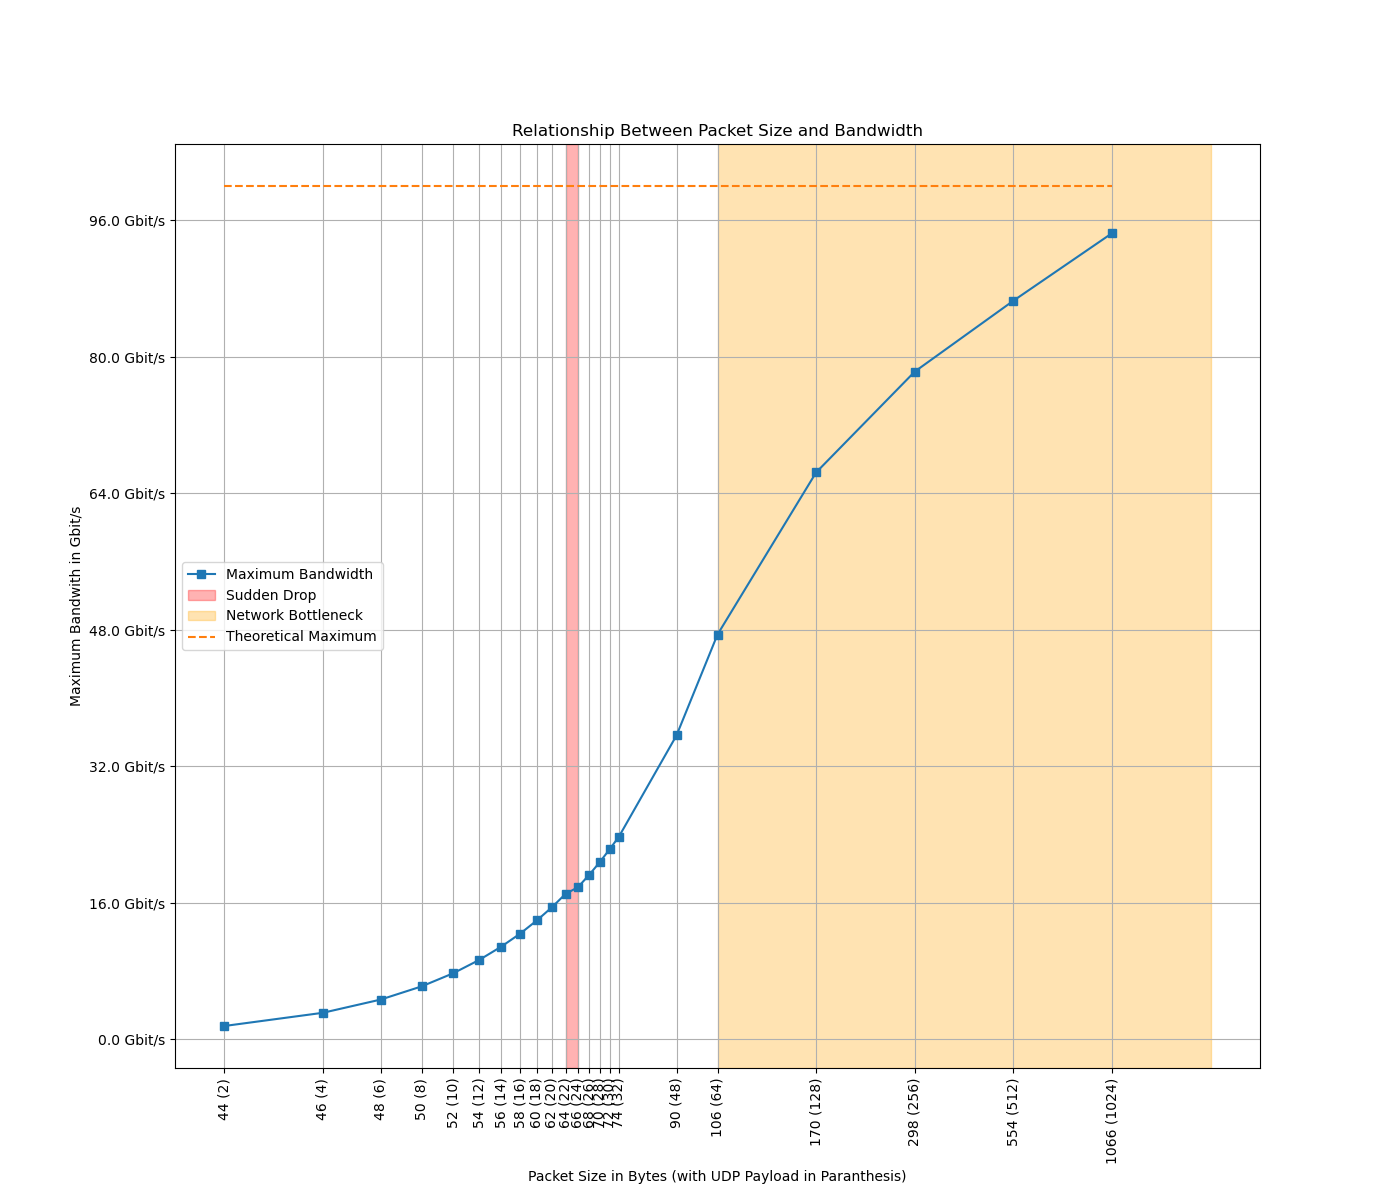
\includegraphics[width=1\linewidth]{images/pps_bandwidth.png}
    \caption{Pakete pro Sekunde - verfügbare Bandbreite}
    \label{fig:enter-label}
\end{figure}
Bei Betrachtung von Abbildung 7.4, in der das Verhältnis zwischen der Paketgröße und der maximalen möglichen Bandbreite abgetragen ist, fällt sofort auf, dass die Erklärung seitens NVidia von angeblichen 400 Gbit/s so nicht nachgewiesen werden konnte. Dies ist vor allem der Tatsache geschuldet, dass in dieser Arbeit vor allem kleine Pakete gemessen wurden. Dennoch liegen die Messungen auch weit unter dem in dem gegebenen Testbed-Netzwerk. So können mit Paketgrößen von 64 Bytes, was eine sehr typische Paketgröße für DNS-Pakete ist, gerade einmal 16 Gbit/s erreicht werden. Dies ist in etwa 4 \% der beworbenen Leistung und somit weit unter der erwarteten Performance. Vergleichen wir allerdings die Leistung zu der eines gängigen Software-Lastverteilers wie Katran in der Arbeit von Phillip Ungrund, so sehen wir eine ungefähr doppelt so hohe Menge von maximalen Paketen pro Sekunde, die verarbeitet werden können \cite{ungrund} (Abbildung 7.5). 

In Abbildung 7.6 ist ein Vergleich zwischen den unterschiedlichen Lastverteilern hinsichtlich ihrer maximalen Pakete/Sekunde Verarbeitungs-Geschwindigkeit. Kakao Corporation ist ein südkoreanischer Cloud-Anbieter, der einen ähnlichen Ansatz verfolgt hat. Es wurde bei deren Versuch ein eBPF-Lastverteiler, ähnlich wie Katran, implementiert \cite{lee2021high}. Dazu wurden aus ihren Messungen zwei entnommen. Im Loopback-Versuch haben sie den eingehenden Traffic eins zu eins wieder ausgegeben und wollten so eine Baseline der maximal möglichen Leistung schaffen. Bei dem 255-Backends-Versuch gab es einen VIP-Server, auf dem die eigentliche Lastverteilung mittels eBPF stattfand. Beide Ansätze sind zwar langsamer als Katran, aber befinden sich bezüglich der maximalen Leistung nahe beieinander. XenoFlow jedoch kann mit einem Speed-Up von über zwei gemessen werden.
\begin{figure}
    \centering
    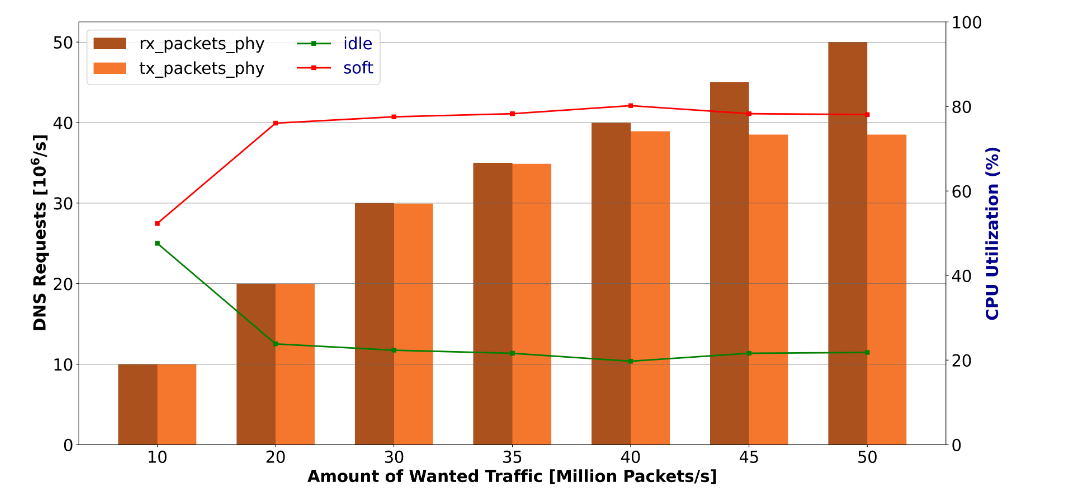
\includegraphics[width=1\linewidth]{images/katran_performance.png}
    \caption{Katran Lastverteiler Leistung bei 254 Quell IP Adressen \cite{ungrund}}
    \label{fig:enter-label}
\end{figure}
\begin{figure}
    \centering
    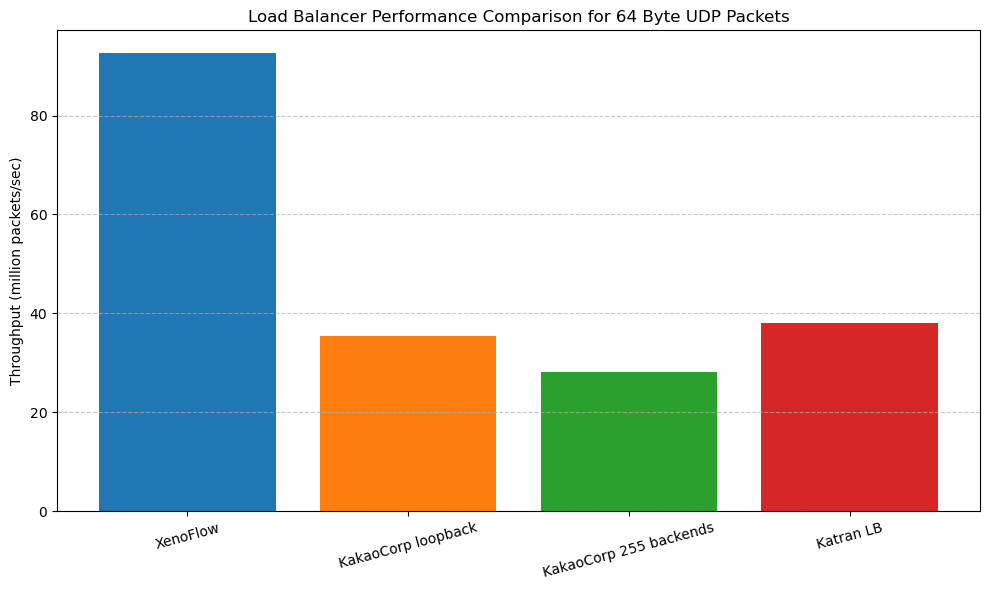
\includegraphics[width=1\linewidth]{images/lb_comp.png}
    \caption{Vergleich von unterschiedlichen Lastverteilern vs. XenoFlow \cite{lee2021high}\cite{ungrund}}
    \label{fig:enter-label}
\end{figure}
\subsection{Latenz}
Die Latenz wurde gemessen, indem zunächst eine Grundlast auf den Lastverteiler ausgeübt wurde. Nun wurde von fips-1 ein einzelner DNS-Request an den Lastverteiler geschickt, der diesen Request aufgrund seiner Source-IP an fips-2 weitergeleitet hat. Fips-2 hat daraufhin eine Antwort an fips-1 mit der IP gesendet. Auf fips-1 wurde dabei die Zeit gemessen, die das Paket für diesen kompletten Pfad gebraucht hat. Dieser Wert wird auch als Round-Trip-Time, kurz RTT, bezeichnet. In dieser Versuchsreihe wurde nun variiert, wie viel des Grundtraffics an die beiden Backends geschickt wird. Dies wird anhand der Source-IP-Felder gesteuert. Somit kann beobachtet werden, ob es Algorithmen gibt, die stochastisch den Traffic verteilen, oder ob es tatsächlich eine Paketverarbeitung für jedes einzelne Paket gibt.
\subsubsection{Single Endpoint}
\begin{figure}
    \centering
    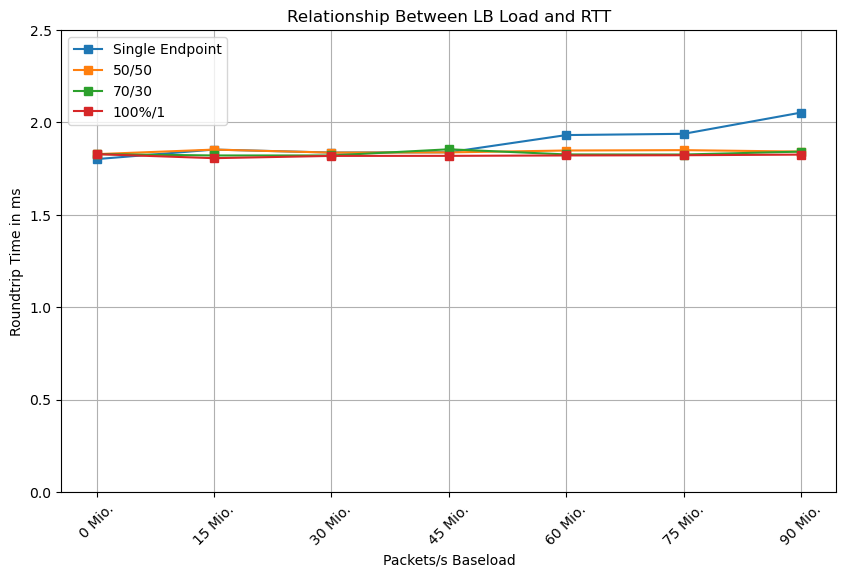
\includegraphics[width=0.9\linewidth]{images/latency.png}
    \caption{Latenzmessungen in unterschiedlichen Szenarien}
    \label{fig:enter-label}
\end{figure}
Bei dem Versuch aus Abbildung 7.7 wird die gesamte Grundlast an den gleichen Server weitergeleitet, auf dem auch der DNS-Server liegt. Hierbei ist der Latenzzuwachs vermutlich durch die Last auf dem Backendsystem zu begründen. Der DNS-Server muss sich mit den restlichen kernelinternen Prozessen um CPU-Zeit streiten, was sich in teilweise schlechteren Antwortzeiten bemerkbar macht. Allerdings ist der Latenzzuwachs sehr gering.
\subsubsection{50/50}

Es ist in Abbildung 7.7 bei einer 50/50-Lastverteilung kein signifikanter Latenzzuwachs in Abhängigkeit von der Basislast zu erkennen.
\subsubsection{70/30}

Es ist in Abbildung 7.7 bei einer 70/30-Lastverteilung kein signifikanter Latenzzuwachs in Abhängigkeit von der Basislast zu erkennen.
\subsubsection{Worstcase}
Bei dem Versuch wird der komplette Netzwerkverkehr außer dem DNS-Request-Paket an das Backend ohne DNS-Server weitergeleitet. Gäbe es einen Zusammenhang mit dem Matching der Pakete und der entsprechenden Verteilung, so würde es bei diesem Versuch vermutlich am ehesten sichtbar werden.
Es ist in Abbildung 7.7 kein signifikanter Latenzzuwachs in Abhängigkeit von der Basislast zu erkennen.
\subsection{Paketverlust}
\begin{figure}
    \centering
    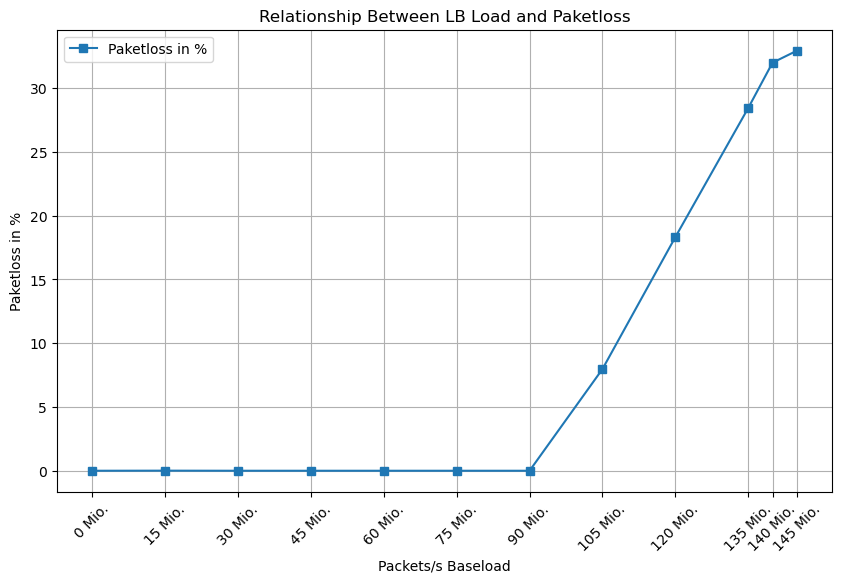
\includegraphics[width=0.95\linewidth]{images/packetloss.png}
    \caption{Paketverlust vs. Pakete pro Sekunde Basislast}
    \label{fig:enter-label}
\end{figure}
In Abbildung 7.8 ist erwartungsgemäß ein lineares Wachstum des Paketverlustes ab der entsprechenden maximalen Verarbeitungsgeschwindigkeit von ca. 95 Millionen Paketen pro Sekunde zu beobachten. Für den entsprechenden Versuch wurden Pakete der Größe 64 Byte verwendet. Somit ist der Paketverlust direkt proportional zu dem im  Versuch der Bandbreite ermittelten maximalen Paketdurchsatz.